\chapter{Experimental results}\label{chapter:Results}
All the tests were performed on a MSI GL63 8RD laptop, using Windows 10 Home version 1909 as Operating System.

\section{Human detection}
The application response was tested over all the three possible scenarios (see \myref{Section}{AcCAPPCHA:user_activity}): 
\begin{itemize}
\item{Time correspondence}
\item{Character correspondence}
\item{Both time and character correspondence}
\end{itemize}
The first method is the most efficient and usually at first or second trial already finds a human activity. Sometimes the correspondence isn't found at first trial because of background noise. \\
The last two approaches based on deep learning require the reduction of the number of labels to obtain good results. In this way I limit the possible characters that user could use and the password should be composed of lower case alphabetic characters, accented vowels or numbers (see \myref{Figure}{Results:keyboard}) but considering again the 10 high probable labels predicted for each peak.\\
In any case the last method that uses both the time and the character correspondence speed up the search of the correct peak related to the insertion and reduces the possibility of having a false positive. However there are many false negatives given by the similar sound produces by several keys opposite to D. Asonov, R. Agrawal's conclusions\cite{keyboard_acoustic}.\\
The reasons of their presence could be:
\begin{itemize}
\item{different parts of my keyboard plate produce similar sounds}
\item{the built-in microphone of my laptop is more affected by the noise than an external microphone}
\item{the movements of the user's hands influence the noise during the password insertion}
%WORN OUT = usurato
\item{some keys are more worn out that other}
The worst deep learning method is the one that uses the spectrograms and a pre-trained deep learning model to extract the features of a press peak. In \myref{Table}{}
However during the insertion of the password, the user can obviously type backslash key but then '$\setminus b$' character isn't considered in the final verification.\\

\end{itemize}
\begin{figure}[h]
     \centering
	 \includegraphics[width=0.8\textwidth]{Images/Results/keyboard_less}
     \caption{\footnotesize{Keys to be used in the password (highlighted in green).}}\label{Results:keyboard}
\end{figure}
\begin{table}[h]
\centering\footnotesize
\begin{tabular}{ccc}
\hline
{\textbf{Feature type}}&{\texttt{\textit{bye5}}}&{\texttt{\textit{hello35}}}\\
\hline
\multirow{3}{*}{FFT of touch peak} & {2 (3/4)} & {1}\\
& {2 (3)} & {1}\\
& {1} & {1}\\
\hline
\multirow{3}{*}{FFT of touch and hit peaks} & {2 (3)/4} & {2 (6/7)}\\
& {2 (3/4)} & {1}\\
& {3 (3/4)} & {3 (5.5/7)}\\
\hline
\multirow{3}{*}{Spectrogram of touch and hit peaks} & {NO (3)} & {NO (5.33/7)}\\
& {NO (2.67/4)} & {NO (6/7)}\\
& {NO (2.67/4)} & {NO (4.67/7)}\\
\hline
\end{tabular}
\end{table}

\section{Bot detection}
I've tested both human and bot activities analysing the response generated by AcCAPPCHA. The bot activity was emulated using several approaches and using the username \texttt{'RaffaDNDM'} and its password \textbf{'hello35'}:
\begin{itemize}
\item{\textbf{Python program with} \texttt{popen} \textbf{communication}\\
this approach opens a subprocess and a communication through pipes with stdin and stdout streams (see ). Assuming the hacker obtained the credentials in some way, the bot communicates the username and the password to running AcCAPPCHA with only time correspondence option selected. In practice the strength of AcCAPPCHA against this attack is very high because the insertion of the password is managed through \texttt{getwch()} call in the Windows Operating system. \\
This function belongs to \texttt{msvcrt} module and takes one character at the time. This module guarantees also that the console I/O routines are not compatible with stream I/O or low-level I/O library routines. In the Windows operating systems, the output from these functions is always directed to the console and cannot be redirected through any king of pipes.\\
The program easily accepts the username, because AcCAPPCHA acquires it using standard \texttt{input()} function. Then AcCAPPCHA waits for characters of password, until ENTER key is pressed, but popen doesn't have access to the stream analysed by \texttt{getwch()}. I didn't iterate the insertion of the password for the maximum number of possible trials because even at the first insertion, AcCAPPCHA doesn't see the insertion of the bot.
\begin{lstlisting}[language=python, showstringspaces=false, tabsize=4, basicstyle=\footnotesize, caption={\footnotesize{Bot using popen.}},label={Results:popen_bot}]
from subprocess import Popen
import sys
import msvcrt
from time import sleep

def popen_bot(username, password):
    #Subprocess that redirects pipes
    process = Popen('python3 AcCAPPCHA.py -t -plot',
    				shell=True, 
    				stdin=subprocess.PIPE,
    				stdout=subprocess.PIPE,
    				stderr=subprocess.STDOUT)

    #Wait until username could be inserted
    sleep(4)
    #Write username and password
    credentials = username.encode() + b'\r\n' + \
    			  password.encode() + b'\r\n'
    output = process.communicate(credentials)[0]
    
    print(output.decode())
\end{lstlisting}
}
\item{\textbf{Python program with} \texttt{pynput} \textbf{module}\\
Using this module, I pretended to be a bot and access directly the console, bypassing the stream limits of \textbf{msvcrt} character acquisition. To emulate the user the bot program should start the execution run and immediately after the hacker must open the working terminal with AcCAPPCHA running.\\
This scenario isn't very feasible because requires management of terminal windows but was useful to establish if the insertion of the password by malicious software is correctly classified as a bot activity. Each character of the password is inserted emulating press and release of the corresponding key of the keyboard.
\begin{lstlisting}[language=python, showstringspaces=false, tabsize=4, basicstyle=\footnotesize, caption={\footnotesize{Bot using pynput module.}},label={Results:pynput_bot}]
from pynput.keyboard import Key, Controller
from time import sleep

def input_bot(username, password):
    #Object for control of keyboard events
    keyboard = Controller()

    def press_release(char):
        keyboard.press(char)
        keyboard.release(char)

    #Wait that username could be inserted
    sleep(4)

    #username insertion
    for x in username:
        press_release(x)
    
    press_release(Key.enter)

    #Trials for password insertion
    count = 0
    while(count<3):
        sleep(5)
        
        for x in password:
            press_release(x)

        press_release(Key.enter)
        count += 1
\end{lstlisting}
}
\item{\textbf{Remote control of the PC}\\
the last test was performed by using the program \texttt{Team Viewer} and accessing directly the terminal. For this reason, this type of attack isn't feasible in practice as the previous mentioned attack with Python bot.}
\end{itemize}
In the last two approaches the audio recorded by AcCAPPCHA are very similar and highlights the two most probable situations:
\begin{itemize}
\descItem{The noise during noise evaluation is very high}{If this happens, no audio peaks can be found (see \myref{Figure}{Results:silence_img}).}
\descItem{The noise during noise evaluation is normal or very low}{If this happens, some audio peaks can be found if there is some noise during password insertion. However they don't have time correspondence with time instants stored during the password insertion (see \myref{Figure}{Results:noise_img}). The only case, in which a bot can authenticate it self, is when there is a sequence of audio peaks caused by the noise and the time between them is the same of the stored ones. However this event isn't very probable because it is hard that there would be too high noise only during the insertion of the password and not during the noise evaluation. For example, if the attacker would analyse the background noise finding a sequence of peaks and defining a model for amount of time between each couple of them, he couldn't use information from it. In fact it could insert a character of the password after an amount time previously modelled but in practice, the peaks of background noise would be discarded through noise evaluation.}
\end{itemize}
\begin{figure}[h]
     \centering
	 \begin{subfigure}[b]{0.48\textwidth}
         \centering
         \includegraphics[width=\linewidth]{Images/Results/Bot/silence}
         \caption{\footnotesize{Bot with \texttt{pynput} module.}}
     \end{subfigure}
	 \hfill     
     \begin{subfigure}[b]{0.48\textwidth}
         \centering
         \includegraphics[width=\linewidth]{Images/Results/TeamViewer/silence}
         \caption{\footnotesize{Team Viewer.}}
     \end{subfigure}
     \caption{\footnotesize{Plot of audio during the password insertion with high noise during noise evaluation.}}\label{Results:silence_img}
\end{figure}
\begin{figure}[h]
     \centering
	 \begin{subfigure}[b]{0.48\textwidth}
         \centering
         \includegraphics[width=\linewidth]{Images/Results/Bot/noise}
         \caption{\footnotesize{Bot with \texttt{pynput} module.}}
     \end{subfigure}
	 \hfill     
     \begin{subfigure}[b]{0.48\textwidth}
         \centering
         \includegraphics[width=\linewidth]{Images/Results/TeamViewer/noise}
         \caption{\footnotesize{Team Viewer.}}
     \end{subfigure}
     \caption{\footnotesize{Plot of audio during the password insertion with low noise during noise evaluation.}}\label{Results:noise_img}
\end{figure}

\section{Usability}
The verification with deep learning techniques would be more strong if the predictions would be more accurate. A problem of this methods is that the neural network must be trained using audio file of keys of a specific keyboard. This method limits the usability of the resulting weights for all the neurons to the specific keyboard previously used. \\
To use the character correspondence on every possible keyboard, each producer of keyboards should record audio produced by pressed keys and share the results to increase the efficiency of AcCAPPCHA. This action should also bring to a malicious use of the data (e.g. an attacker could use them to produce an advanced key-logger).\\
I used also other input devices to test the usability of the best method (time correspondence). At first I tested AcCAPPCHA using an external wireless keyboard (Logitech K480) by positioning it in front of my laptop. I tested AcCAPPCHA using touch keyboard and one the following hardware devices:
\begin{itemize}
\descItem{Mouse}{this device guarantees to perform the time correspondence exploiting the sound of each mouse click needed to select a key.}
\descItem{Touchpad}{this device also guarantees to perform the time correspondence exploiting the sound of each click the touchpad needed to select a key. The only condition, required by AcCAPPCHA to work correctly, is that the user clicks the physical left button at the bottom side of the touchpad.}
\end{itemize}
The results of verification using these three devices were the same of the ones obtained using the keyboard of the laptop.

\section{Security analysis}\label{Results:security}
Following the analysis performed for Invisible CAPPCHA\cite{Invisible_CAPPCHA}, I'm going to discuss the strength of AcCAPPCHA against the following attacks:
\begin{itemize}
\descItem{Replay attack}
{The message is still concatenated with a nonce and then they are signed to guarantee a client would use a nonce only one. The server still prevents this type of attacks by refusing the second message from a client with a nonce already used by him.}
\descItem{Reverse engineering attack}
{The code working on the client must be kept secure by the File System. Even if the attacker could reverse code on server, the signature of the message and the TLS communication guarantee that this attack cannot be performed.}
\descItem{Human-solver relay attack}
{AcCAPPCHA is strong there aren't additional tasks to be performed as in classical CAPTCHAs. Hence no challenges can be sent to remote human solver.}
\descItem{Brute force and password replay attacks}
{at the contrary of Invisible CAPPCHA, a single call to AcCAPPCHA performs the verification of human identity for at most 3 times:
\begin{itemize}
\descItem{if a bot is detected in one of the 3 attempts}{the program asks again the password to the user and reduces the number of remaining trials}
\descItem{Otherwise}{the password inserted by the user is compared with the one in the database. In any case, the client program terminates receiving an HTML page with the result of the login phase.}
\end{itemize}
The server doesn't know if AcCAPPCHA was called more than once by the client. If the server wants to allow no more than a fixed amount of attempts, it could count the number of POST requests received during a fixed amount of time by each client. If the number of requests reaches the maximum number of designed attempts, the server adds the corresponding client to a black list and then communicates it to the client. Hence the client-side of AcCAPPCHA, receiving the message from server, will refuse next attempts of verification (insertion of password).
}
\descItem{Denial Of Service (DOS)}
{For the same reason previously explained, the number of passwords received by the server is 1. To prevent a DOS attack, the server could use the same approach with black list designed to prevent the previous attack. In fact the server won't be overloaded, because the client will refuse next attempts.}
\end{itemize}
If an attacker has remote control of the pcon which client-side AcCAPPCHA can run, the user could understand on Windows 10 that he's under attack by looking the microphone icon on the taskbar. In fact, I suggest every user to enable this icon in \textbf{Settings > Personalisation > Taskbar > Turn system icons on or off} even if an attacker could disable it. Every time that an application accesses the microphone resource, the user could see the icon on the taskbar if it was enabled on the settings.   